Esse capítulo introduz a infraestrutura para realização dos testes, quais foram os experimentos realizados e as métricas utilizadas. Também apresenta os resultados dos experimentos e as conclusões geradas a partir da análise dos dados coletados.

\section{Infraestrutura e parâmetros}

Para a realização dos experimentos e validação dos resultados foi utilizada uma máquina virtual hospedada no software \textit{Kernel-based Virtual Machine} (KVM) sobre o sistema operacional \textit{TrueNAS Scale}\footnote{https://www.truenas.com/truenas-scale/}.
A máquina virtual executa o sistema operacional Ubuntu Server 20.04.4 LTS e possui diferentes configurações de processador e memória RAM, variando entre 4, 6, 8 e 12 núcleos virtuais de um processador \textit{Intel Core i7 8700T}, 4 e 8 GB de memória RAM DDR4-2666 e um disco virtual de 64 GB armazenado em um SSD M.2 NVMe.
Detalhes resumidos da máquina virtual podem ser consultados na Tabela \ref{tab:vm-config}.

Para a execução dos experimentos, foi criada uma imagem de base da máquina virtual pré-configurada, que era restaurada ao fim de cada execução do experimento, evitando que resquícios de uma execução anterior pudessem afetar outras execuções do experimento.
Além disso, também foi utilizado o sistema de conteinerização \textit{Docker}\footnote{https://www.docker.com/} para isolar os componentes do núcleo da rede 5G e do testador.

% Please add the following required packages to your document preamble:
% \usepackage{multirow}
\begin{table}[!ht]
\centering
\caption{Configuração da máquina de testes}
\label{tab:vm-config}
\begin{tabular}{|l|cccc|}
\hline
                                      & \multicolumn{4}{c|}{\textbf{Máquinas Virtuais}}    \\ \hline
\multirow{2}{*}{\textbf{CPU}}         & \multicolumn{4}{c|}{Intel Core i7 8700T @ 2.4 GHz} \\ \cline{2-5} 
 & \multicolumn{1}{c|}{4 núcleos} & \multicolumn{1}{c|}{6 núcleos} & \multicolumn{1}{c|}{8 núcleos} & 12 núcleos \\ \hline
\multirow{2}{*}{\textbf{Memória RAM}} & \multicolumn{4}{c|}{DDR4 2666 MHz}                 \\ \cline{2-5} 
 & \multicolumn{1}{c|}{4 GB}      & \multicolumn{1}{c|}{8 GB}      & \multicolumn{1}{c|}{8 GB}      & 8 GB       \\ \hline
\textbf{Armazenamento}                & \multicolumn{4}{c|}{SSD M.2 64 GB NVMe}            \\ \hline
\textbf{Sistema Operacional}          & \multicolumn{4}{c|}{Ubuntu Server 20.04.4 LTS}     \\ \hline
\end{tabular}
\end{table}

Dois experimentos distintos foram realizados sobre diferentes configurações dessa infraestrutura.
Os experimentos foram os testes de tempos de registro e estabelecimento de sessão do núcleo 5G e testes de desempenho do plano de dados do núcleo 5G.

\subsection{Testes de tempos de registro e estabelecimento de sessão do núcleo 5G}

O experimento para medição de tempos de registro e estabelecimento de sessão do núcleo 5G consiste na simulação de múltiplos UEs tentando se conectar e estabelecer uma sessão PDU com o núcleo 5G a ser testado.
Desse modo, é possível medir a latência entre cada estágio da conexão e sua variação de acordo com a carga de trabalho aplicada sobre o núcleo.
Para que fosse possível medir essa latência em diferentes cenários de forma automatizada, foi adicionado parâmetros de configuração tanto no orquestrador do experimento quanto no módulo de testes.
Neste experimento, também foram coletadas as métricas de uso de processador, memória RAM, disco e rede de todos os componentes do núcleo da rede 5G e do testador, utilizando-se as ferramentas para exportação de métricas dos contêineres \textit{Docker}.

Para esse experimento, foi utilizada a configuração da máquina virtual com 12 núcleos virtuais e 8 GB de memória RAM.
Em relação às configurações do experimento, foram utilizadas as versões dos núcleos 5G \textit{free5GC} v3.2.1, sendo a mais recente disponível no momento da execução dos experimentos e \textit{Open5GS} v2.3.6, que é a versão recomendada pelos desenvolvedores do testador.
Para cada núcleo, foram usadas as seguintes configurações do testador: número de gNB variando de 1 a 11, com passo de 2, intervalo entre conexões de 100 ms até 500 ms, com passo de 100 ms e cada gNB conectando 100 UEs.
Esse experimento foi executado 10 vezes, para obter-se uma quantidade de dados relevantes, onde ruídos externos ao experimento fossem amenizados.

Durante os testes para a realização desse experimento, algumas limitações foram encontradas e devem ser ressaltadas.
Primeiramente, pretendia-se utilizar a versão do núcleo \textit{free5GC} v3.0.6, que é recomendada pelos desenvolvedores do testador. Entretanto, essa versão do núcleo apresentou falhas após conectar aproximadamente 10 UEs, o que inviabilizaria a execução desse experimento.
O núcleo OAI apresentou uma limitação parecida tanto na versão v1.3.0, que é recomendada para o testador, quanto na versão v1.4.0, que é a mais recente disponível até o presente momento, falhando após conectar exatamente 15 UEs.
O núcleo \textit{Open5GS} na versão v2.3.6 consegue conectar exatamente 1024 dispositivos simultâneos antes de apresentar erros na função de rede AMF. Sendo assim, foi decidido que o limite de gNBs seria 11, com o total de 1100 UEs sendo conectados, atingindo a limitação desse núcleo.


\subsection{Testes de desempenho do plano de dados do núcleo 5G}

O experimento para medição do desempenho do plano de dados do núcleo 5G consiste na simulação de 1 ou mais UEs realizando o registro no núcleo da rede e iniciando um plano de dados. Após o registro ser concluído, é medida a capacidade do plano de dados utilizando-se a ferramenta \textit{iPerf}\footnote{https://iperf.fr/} versão 2.0.

Para a execução desse experimento, foi decidido utilizar a versão 2.0 da ferramenta \textit{iPerf} ao invés da versão mais recente devido a capacidade da versão 2.0 suportar múltiplas conexões de clientes em uma única instância do servidor, além de permitir exportar as métricas do experimento em um arquivo de texto separado por vírgula, facilitando o pós processamento dos dados.
Em relação à máquina virtual utilizada, foram feitos testes variando o número de núcleos virtuais de processador entre 4, 6, 8 e 12 núcleos virtuais e variando a capacidade de memória RAM entre 4 GB e 8 GB. Cada variação na quantidade de núcleos virtuais possuía uma única configuração de memória RAM. Os detalhes das máquinas virtuais estão declarados na Tabela \ref{tab:vm-config}. 
Nesse experimento, a principal métrica a ser observada é a largura de banda, em \textit{Bytes} por segundo (Bps), representando a capacidade máxima de tráfego de dados entre o UE e a rede 5G, passando pelo componente do núcleo UPF.
Nesse experimento, também foram coletadas as métricas de uso de processador, memória RAM, disco e rede de todos os componentes do núcleo da rede 5G e do testador, utilizando-se as ferramentas para exportação de métricas dos contêineres \textit{Docker}.

Em relação aos parâmetros usados para a execução do experimento, foi utilizada a configuração de 1, 2, 4, 6, 8 e 10 gNBs com 1 UE cada registrando e conectando o plano de dados antes da execução de cada teste de desempenho. Quanto aos parâmetros da ferramenta \textit{iPerf}, foi definido o tempo de execução do experimento em 60 s, reportando as métricas do teste a cada segundo.
Os núcleos de rede 5G testados foram o \textit{free5GC} v3.0.6 e o \textit{Open5GS} v2.3.6, ambas recomendadas pelo testador.
Esse experimento foi executado 16 vezes, para obter-se uma quantidade de dados relevantes, onde ruídos externos ao experimento fossem amenizados.

Algumas limitações foram observadas durante a preparação e execução desse experimento.
Visto que no experimento anterior foi utilizada a versão mais recente do núcleo \textit{free5GC}, havia a intenção de se utilizar a mesma versão para esse experimento. Porém os tutoriais para a implantação da versão v3.2.1 falharam ao estabelecer as rotas necessárias para o plano de dados, inviabilizando a conexão entre o cliente e o servidor do \textit{iPerf}. Desse modo, foi decidido utilizar uma versão anterior deste núcleo, que havia sido homologada pelos desenvolvedores do testador.
Nesse experimento, o OAI apresentou o mesmo problema, com falhas ao estabelecer as rotas entre o UE e a rede 5G nas versões v1.3.0 e v1.4.0, sendo esta a mais recente ate o presente momento. Dessa forma, foi decidido não realizar os experimentos sobre esse núcleo.


\section{Análise e discussão dos tempos de registro e estabelecimento de sessão do núcleo 5G}
Para o experimento de medição do tempo de conexão de equipamentos de usuário, foi levado em consideração o tempo total entre o início do processo de registro e a obtenção do plano de dados. Após a coleta e processamento dos dados desse experimento, os gráficos da Figura \ref{fig:exp1_conn} foram gerados para permitir a visualização e análise dos dados coletados.
O gráfico representa o tempo médio de conexão para cada rajada de conexões simultâneas, com o eixo X representando o tempo de execução do experimento, em segundos, e o eixo Y representando o tempo total para estabelecer a conexão e iniciar o plano de dados deste equipamento de usuário, em milissegundos.
Na coluna da esquerda, são apresentados os resultados para o núcleo 5G \textit{free5GC} e, na direita, o \textit{Open5GS}. Para cada núcleo, foram desenhados 5 gráficos, com as diferentes variações de intervalo entre rajadas de conexões de UEs.

Ao analisar os dados, é possível inferir que, para as condições do experimento, o núcleo \textit{free5GC} possuiu tempo de conexão médio de 1089 ms, quando cada conexão se iniciou 500 ms após a anterior.
Nesse experimento, a mediana do tempo de conexão foi de 853 ms e o tempo máximo de conexão foi de 5,57 segundos.
Para um intervalo entre conexões de 100 ms, o tempo médio de conexão foi de 7731 ms, tendo sua mediana em 3027 ms e o tempo máximo de conexão durando pouco mais de 54 segundos.

Quanto ao comportamento do núcleo de rede 5G \textit{Open5GS}, percebe-se que para um intervalo de 500 ms, o tempo médio foi de 306 ms, com sua mediana em 305 ms e seu tempo máximo de conexão em 345 ms.
Para o intervalo de 100 ms, a média subiu para 364 ms, enquanto a mediana subiu para 358 ms e o valor máximo atingiu 490 ms.
Desse modo, considerando-se apenas o tempo de conexão, o núcleo de rede \textit{Open5GS} possui melhor desempenho, aguentando diversas rajadas de conexões em diferentes cenários, tendo seu tempo médio variando em torno de 58 milissegundos. O núcleo \textit{free5GC} possui uma variação de aproximadamente 49 segundos entre as diferentes execuções do experimento.
Os dados detalhados para cada execução desse experimento podem ser vistos na Tabela \textcolor{red}{INSERIR TABELA}.

\begin{figure}[H]
    \centering
    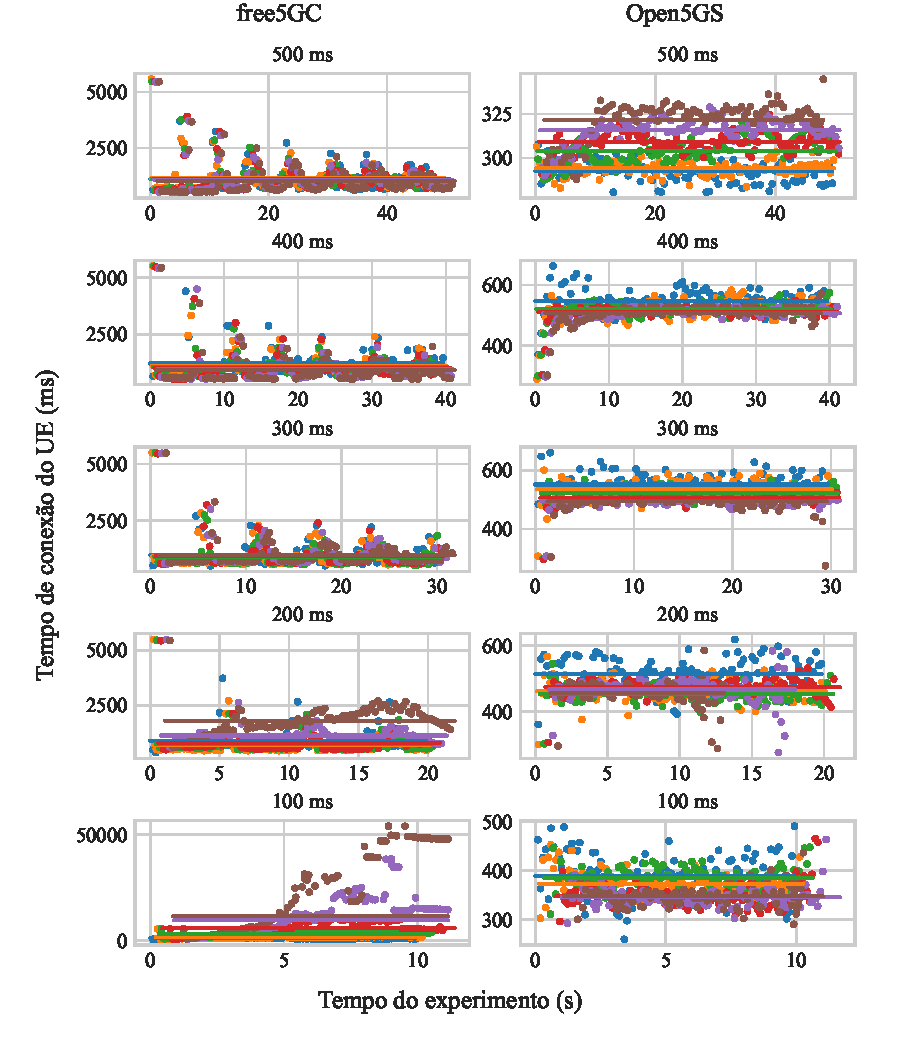
\includegraphics[width=0.85\textwidth]{TG2/Chapters/DataAnalysis/Figures/EXP1-CONN-12C-8GB.pdf}
    \caption{Tempo de registro e estabelecimento de sessão PDU para cada núcleu 5G}
    \label{fig:exp1_conn}
\end{figure}

Durante a execução dos experimentos, a taxa de conexões mal sucedidas entre o UE e o núcleo da rede foi significativa entre cada execução do experimento para cada um dos núcleos testados. Sendo assim, foi desenhado os gráficos da Figura \ref{fig:exp1_conn_err} com a comparação de taxa de erro média entre os dois núcleos avaliados.
Cada gráfico representa a taxa de erro média de conexão dos UEs com os núcleos testados, com o intervalo de tempo entre as rajadas em ordem decrescente, de 500 a 100 ms, com passos de 100 ms.
As barras dos gráficos representam a média de erros entre as execuções do experimento realizadas para cada configuração de gNB e núcleo, enquanto as linhas representam o desvio padrão da média para cada execução do experimento.

Nesse experimento, foi possivel observar que o núcleo \textit{free5GC} possui uma taxa de erros de conexão crescente para cada gNB adicionada. Ao adicionar uma gNB, a taxa de conexões simultâneas aumentava na mesma proporção que a taxa de erros.
Esse comportamento pode ser percebido no núcleo \textit{Open5GS} quando se reduz o intervalo entre rajadas de conexões para um valor menor que o tempo médio necessário para se estabelecer a conexão.
Entretanto, para intervalos maiores de tempo, o núcleo \textit{Open5GS} apresentou boa estabilidade no geral, tendo em alguns momentos a taxa de erros de conexão igual a zero.

Através da análise desses resultados, percebe-se que o núcleo de rede 5G \textit{Open5GS} possui maior estabilidade para o registro de sessões dos UE em escala em comparação com o núcleo \textit{free5GC}.
Apesar desses resultados, foi descoberta uma limitação no núcleo \textit{Open5GS} em relação à quantidade máxima de dispositivos conectados simultaneamente, sendo essa igual a 1024 dispositivos.
É importante ressaltar que essa limitação não está presente no núcleo \textit{free5GC}.
Os dados detalhados para cada execução desse experimento podem ser vistos na Tabela \textcolor{red}{INSERIR TABELA - TALVEZ SEJA A MESMA DE CIMA}.

\begin{figure}[H]
    \centering
    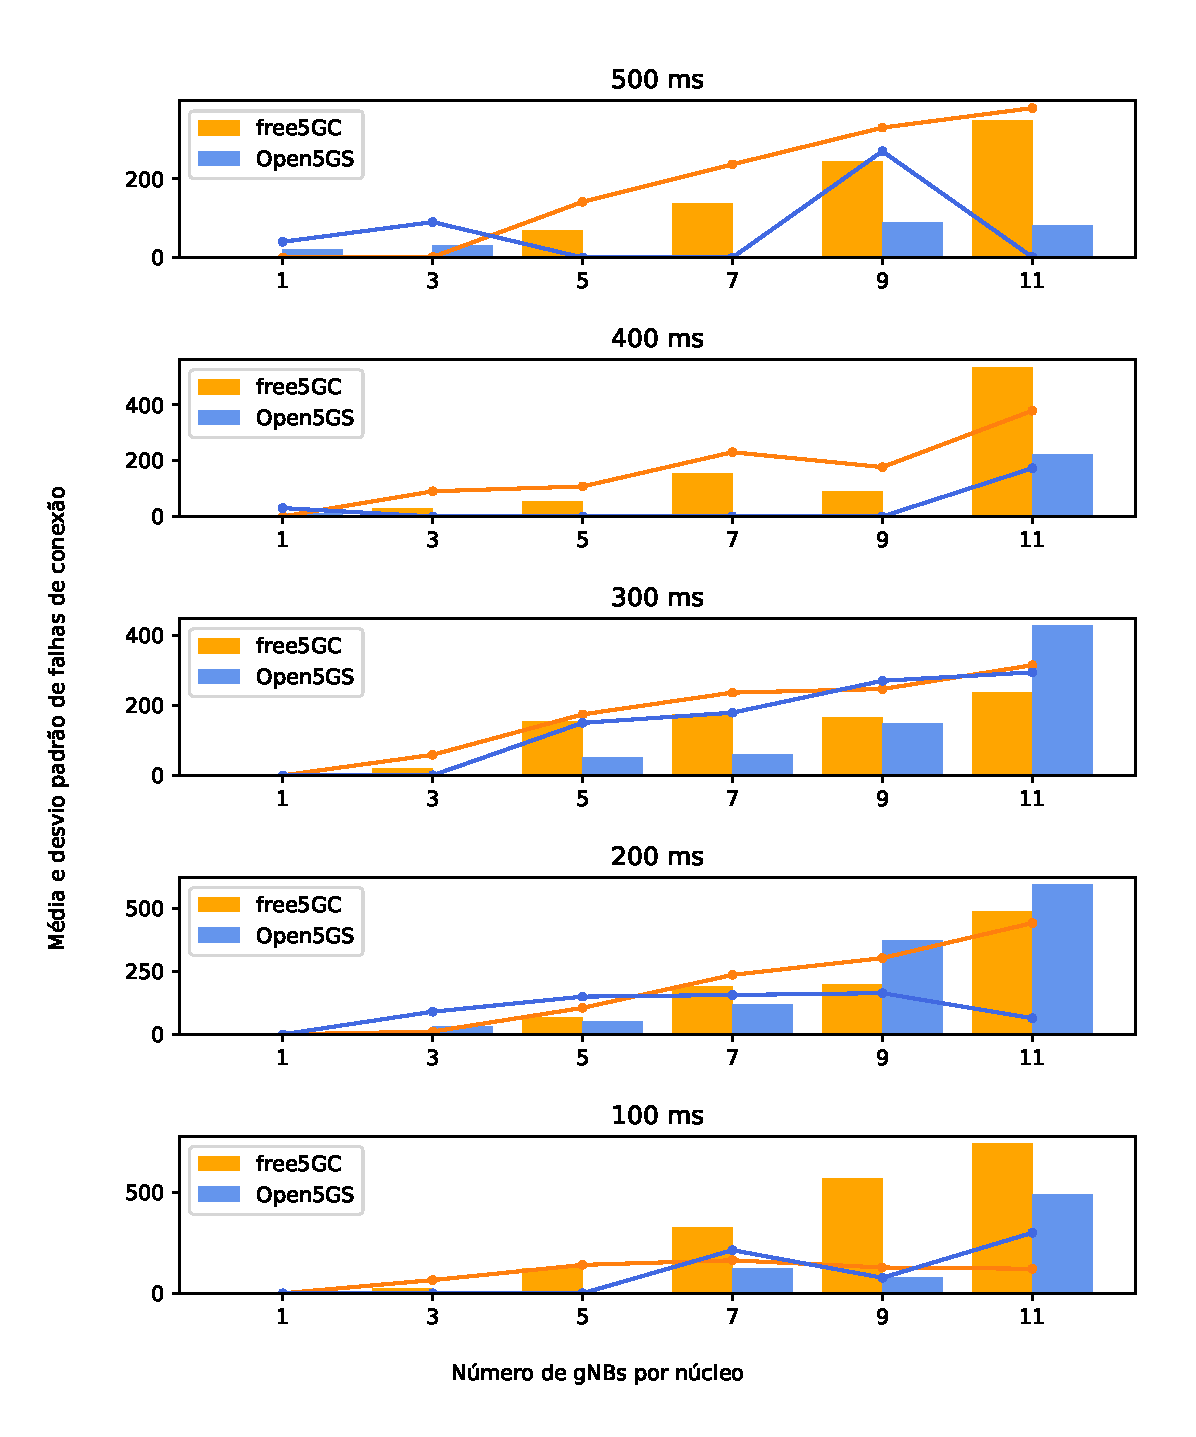
\includegraphics[width=0.95\textwidth]{TG2/Chapters/DataAnalysis/Figures/EXP1-CONN_ERR-12C-8GB.pdf}
    \caption{Média e desvio padrão dos erros de conectividade nos experimentos executados}
    \label{fig:exp1_conn_err}
\end{figure}


\section{Análise e discussão dos resultados em relação ao desempenho do plano de dados}
Para o experimento de avaliação do desempenho do plano de dados do núcleo da rede 5G, foi executada, por 60 segundos, a ferramenta \textit{iPerf} 2.0 simultaneamente em cada UE conectado ao núcleo 5G.
Em um primeiro momento, foi utilizada a máquina virtual em sua configuração máxima, com 12 núcleos virtuais de CPU e 8 GB de memória RAM.
Após a coleta e o processamento dos dados gerados pela ferramenta \textit{iPerf}, foram gerados os gráficos representando a largura de banda por segundo dos núcleos de rede 5G \textit{free5GC} e \textit{Open5GS} testados.

A Figura \ref{fig:exp2_free5gc_12-8} apresenta os gráficos com a largura de banda para cada configuração de quantidade de UE para o núcleo \textit{free5GC} na máquina virtual com 12 núcleos virtual de processador e 8 GB de memória RAM.

\begin{figure}[H]
    \centering
    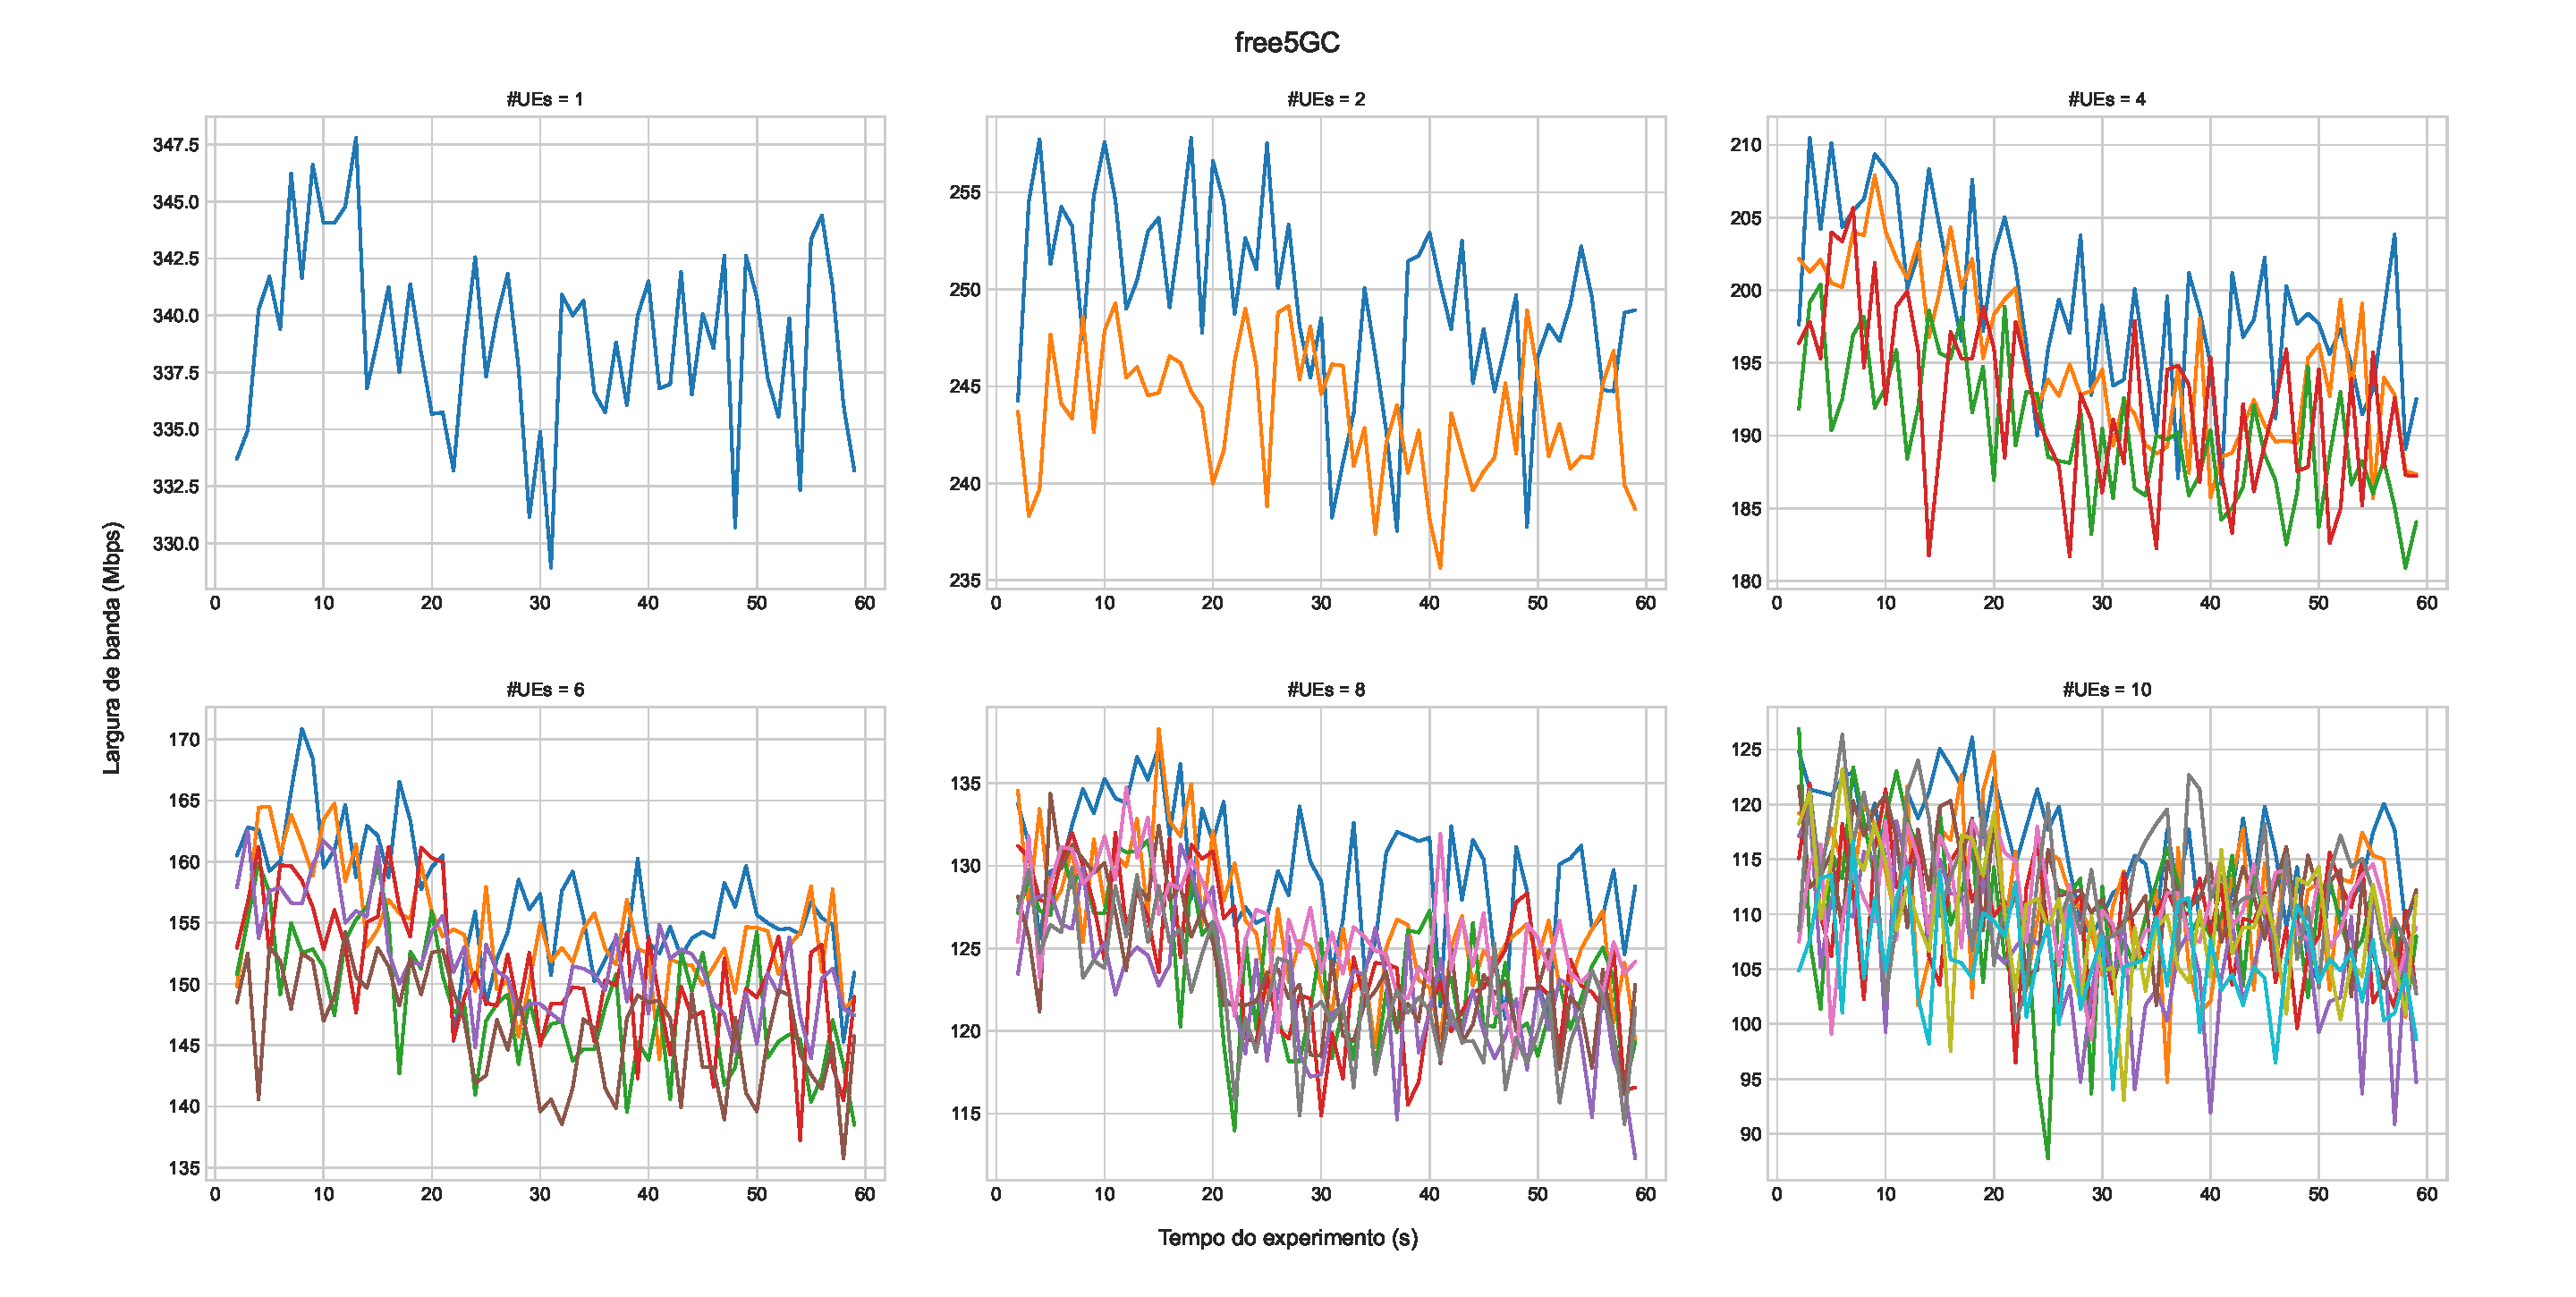
\includegraphics[width=1\textwidth]{TG2/Chapters/DataAnalysis/Figures/EXP2-free5GC-12C-8GB.pdf}
    \caption{Largura de banda para cada configuração de quantidade de UE para o núcleo \textit{free5GC}}
    \label{fig:exp2_free5gc_12-8}
\end{figure}

A Figura \ref{fig:exp2_open5gs_12-8} apresenta os gráficos com a largura de banda para cada configuração de quantidade de UE para o núcleo \textit{Open5GS} na máquina virtual com 12 núcleos virtual de processador e 8 GB de memória RAM.

\begin{figure}[H]
    \centering
    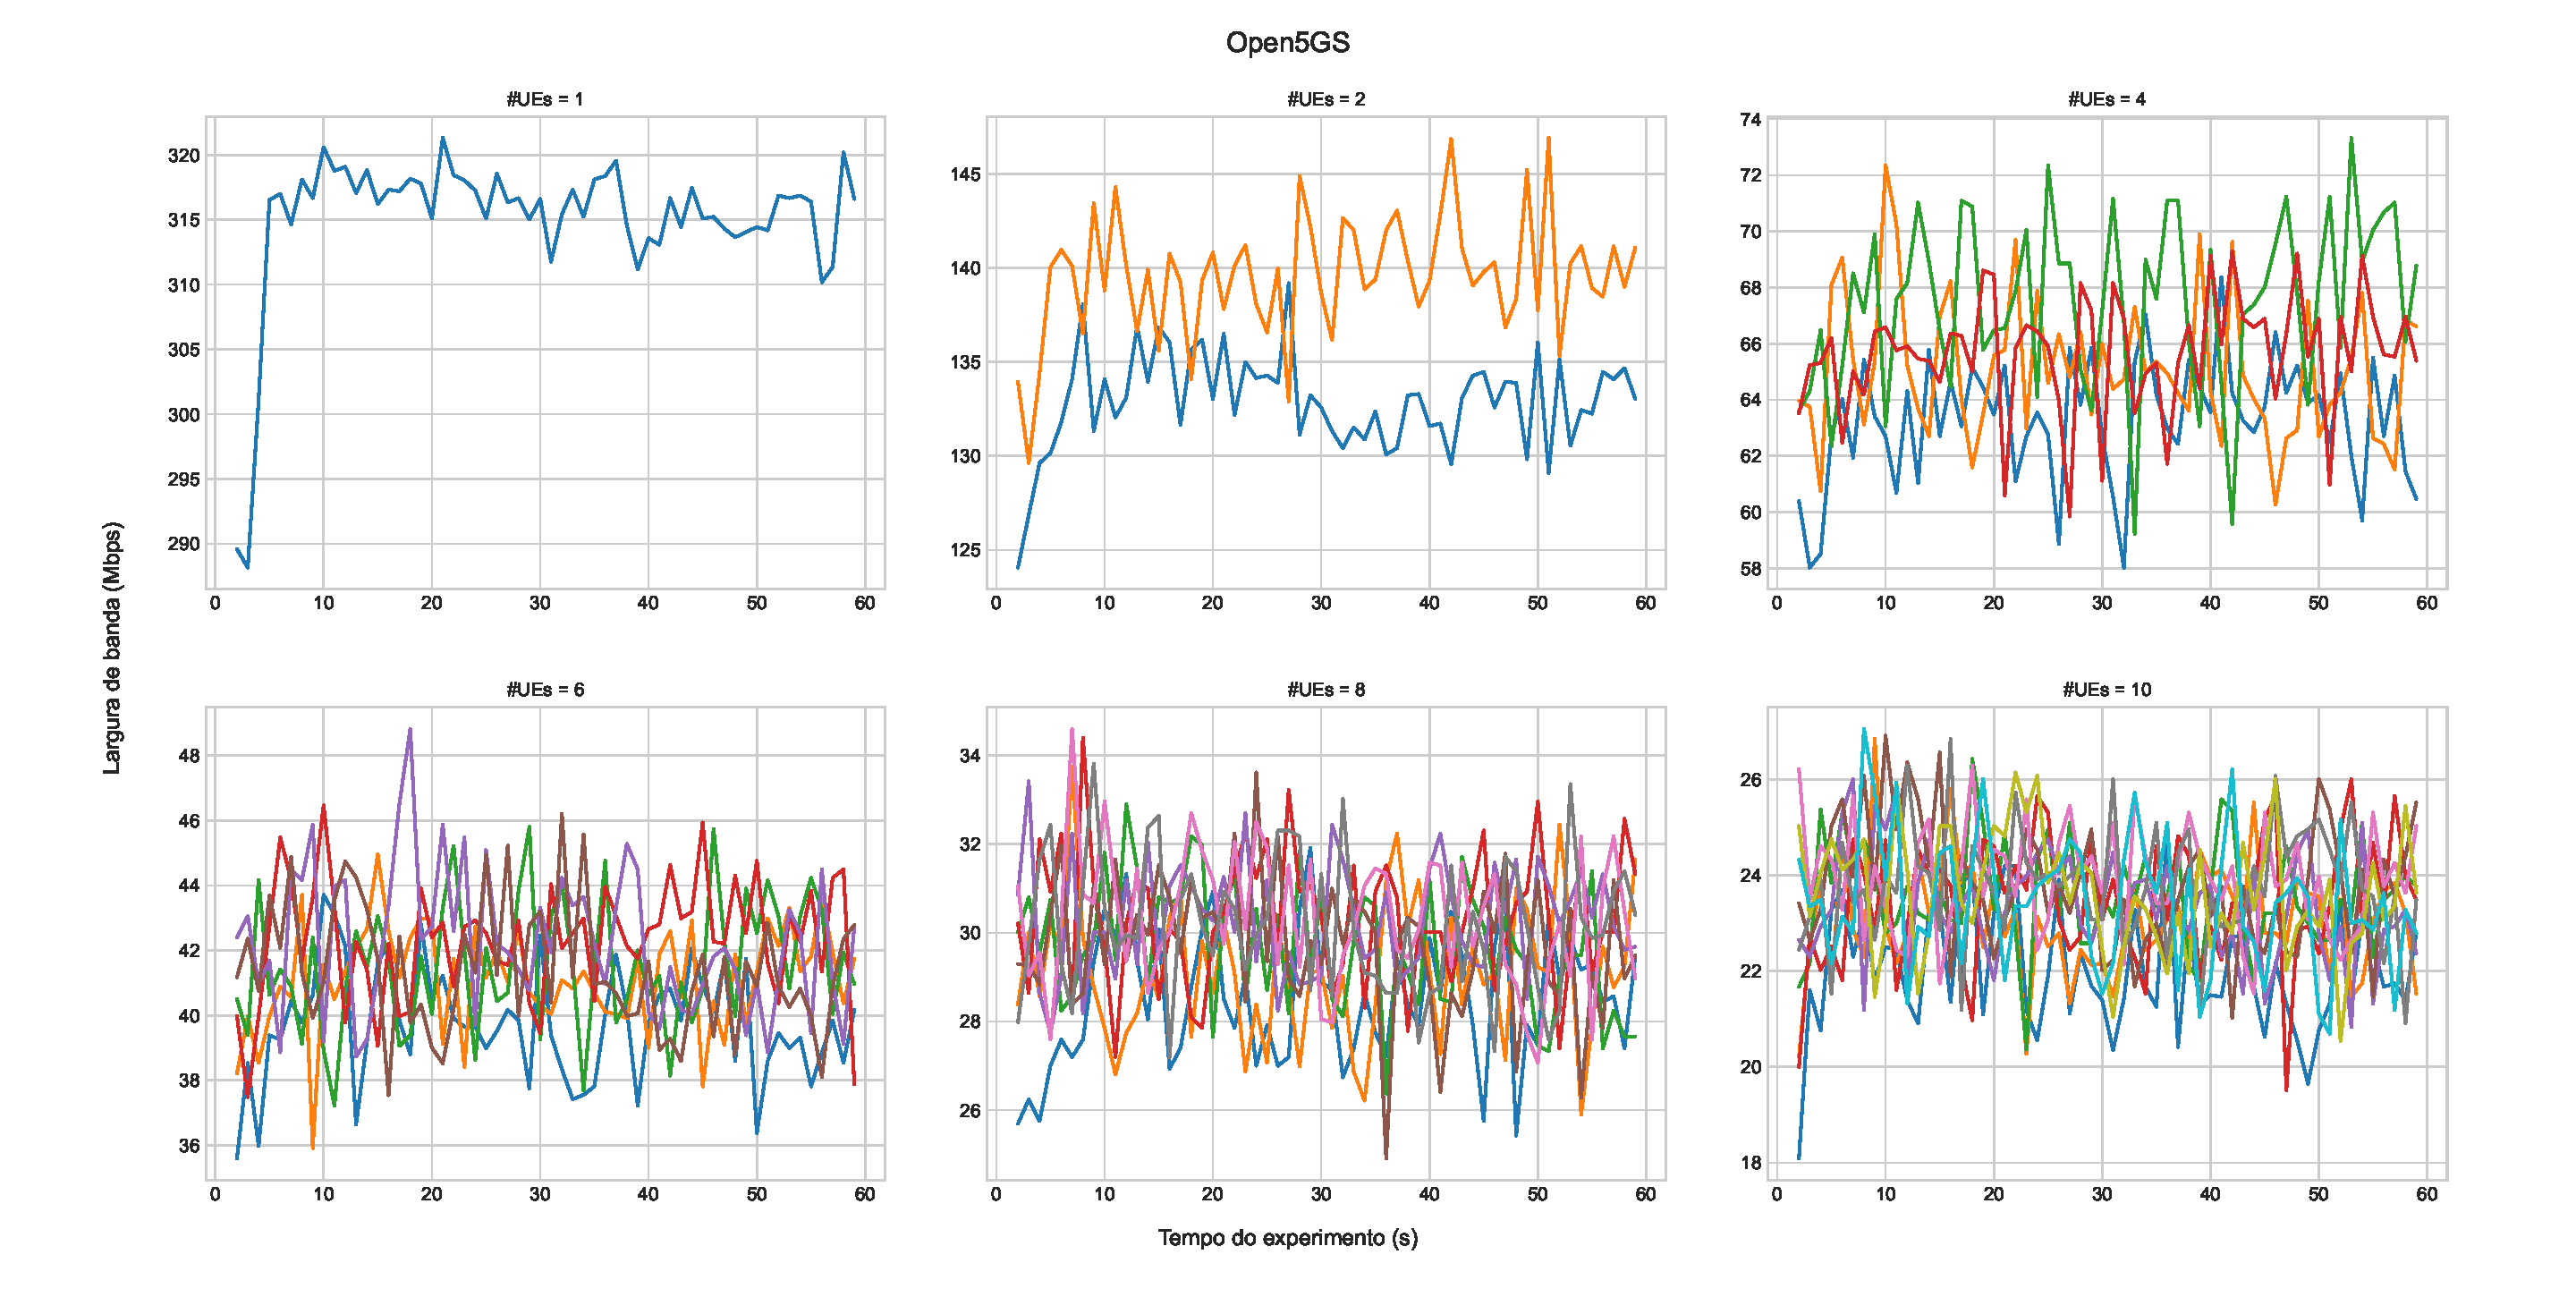
\includegraphics[width=1\textwidth]{TG2/Chapters/DataAnalysis/Figures/EXP2-Open5GS-12C-8GB.pdf}
    \caption{Largura de banda para cada configuração de quantidade de UE para o núcleo \textit{Open5GS}}
    \label{fig:exp2_open5gs_12-8}
\end{figure}

Através desses gráficos, é possível observar que a largura de banda disponível para os UEs não é estável, oscilando durante toda a execução do experimento.
Para uma melhor visualização dos valores agregados de cada execução desse experimento, foram criados gráficos de barra.
O eixo X do gráfico representa o número de UEs em cada rodada do experimento, onde segmento da barra representa o UE de mesma cor das duas figuras anteriores.
Cada barra do gráfico representa a largura de banda média em Mbps agregada entre os UEs.
A Figura \ref{fig:exp2_all_12-8} apresenta o valor agregado da largura de banda para cada configuração de quantidade de UE para a máquina virtual com 12 núcleos virtuais e 8 GB de memória RAM.

\begin{figure}[H]
    \centering
    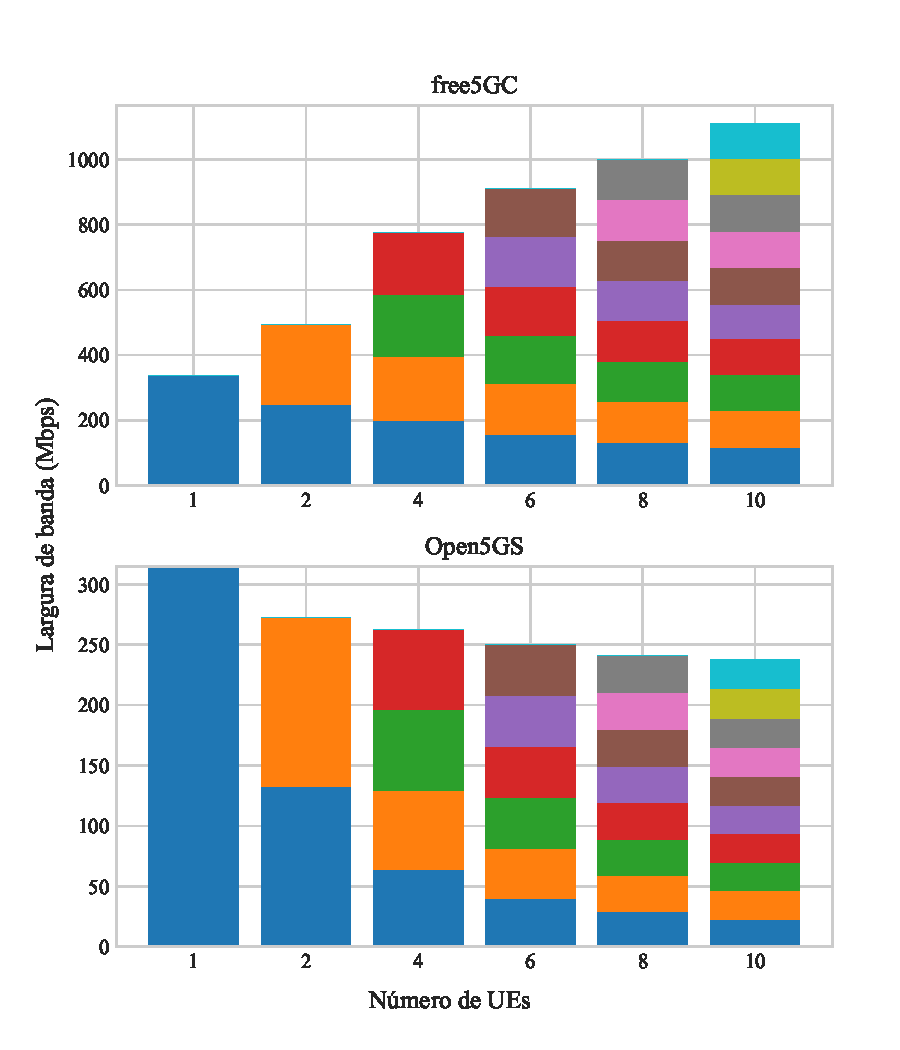
\includegraphics[width=1\textwidth]{TG2/Chapters/DataAnalysis/Figures/EXP2-ALL-12C-8GB.pdf}
    \caption{Valor agregado da largura de banda para cada configuração de quantidade de UEs}
    \label{fig:exp2_all_12-8}
\end{figure}

Nesse experimento, percebe-se que no núcleo \textit{free5GC} a largura de banda total entre cada execução aumenta de acordo com a quantidade de UEs conectados.
O valor médio de largura de banda para esse núcleo com um UE conectado é de 338.4 Mbps, aumentando para 777.0 Mbps com quatro UEs conectadas e 1109.9 Mbps com 10 UEs conectadas.
Em contrapartida, o comportamento do núcleo \textit{Open5GS} se opõe ao \textit{free5GC}. No núcleo \textit{Open5GS}, o valor médio da largura de banda para um UE conectado é de 314.5 Mbps, reduzindo para 262.7 Mbps com 4 UEs conectadas e 237.9 Mbps ao conectar 10 UEs simultâneas.
Esse experimento demonstra que o núcleo \textit{free5GC} possui melhor estrutura para gerenciar o tráfego de dados de UEs em escala em relação ao núcleo \textit{Open5GS}.

Ao limitar a quantidade de recursos disponíveis para a execução do experimento, diminuindo a quantidade de núcleos virtuais de processador e memória RAM da máquina virtual, percebe-se que o desempenho do plano de dados para o núcleo \textit{free5GC} é diretamente proporcional à quantidade de núcleos virtuais disponíveis.
A Figura \ref{fig:exp2_all_8-8} representa o desempenho médio agregado do plano de dados para a execução do experimento em uma máquina virtual com 8 núcleos virtuais de processador e 8 GB de memória RAM.
Nesse caso, largura de banda máxima do plano de dados para o núcleo \textit{free5GC} é reduzida para 1004.2 Mbps quando executado com dez UEs simultâneos.
Essa redução de desempenho pode ser explicada devido à limitação na carga máxima de processamento suportada pela máquina virtual.

\begin{figure}[H]
    \centering
    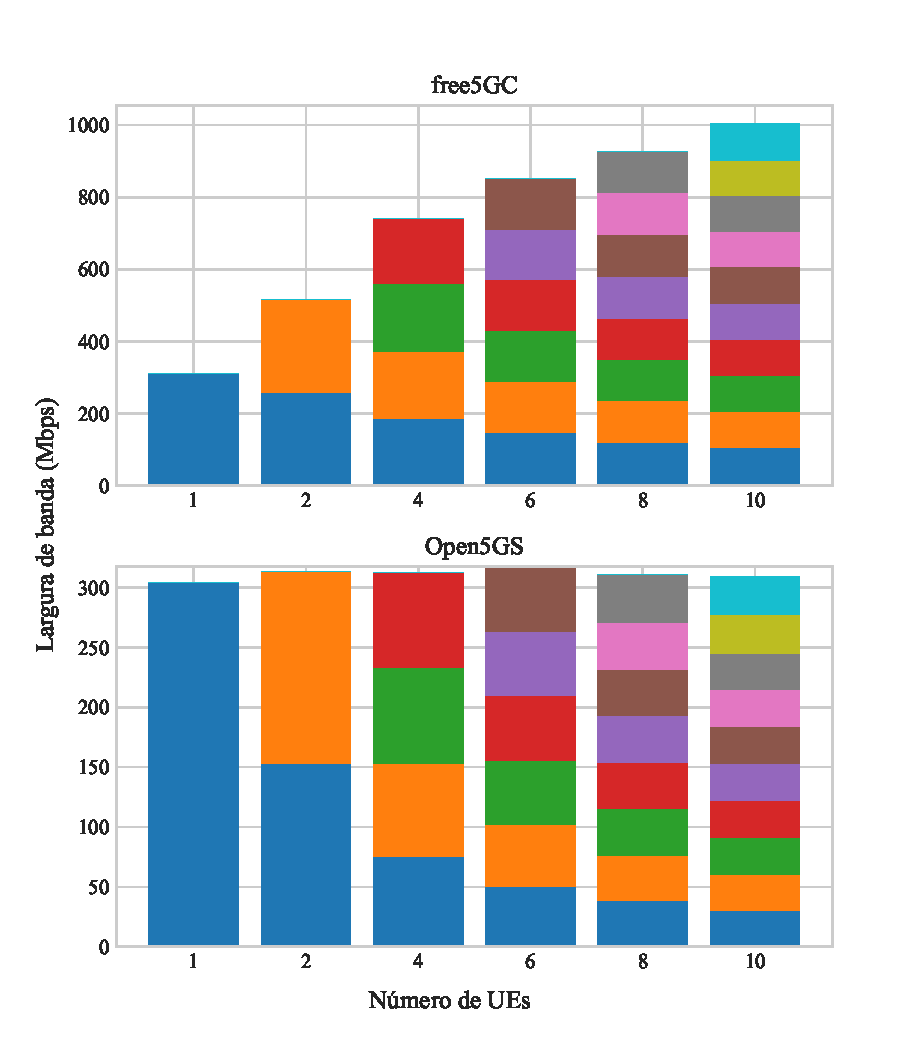
\includegraphics[width=1\textwidth]{TG2/Chapters/DataAnalysis/Figures/EXP2-ALL-8C-8GB.pdf}
    \caption{Valor agregado da largura de banda para cada configuração de quantidade de UEs}
    \label{fig:exp2_all_8-8}
\end{figure}

A redução de desempenho do plano de dados fica mais visível ao limitar-se ainda mais a quantidade de núcleos virtuais disponíveis para o experimento.
Na Figura \ref{fig:exp2_all_6-8}, onde a máquina virtual é executada com 6 núcleos virtuais de processador e 8 GB de memória RAM, é possível perceber que o desempenho máximo do plano de dados do núcleo \textit{free5GC} é atingido com seis UEs simultâneos.

\begin{figure}[H]
    \centering
    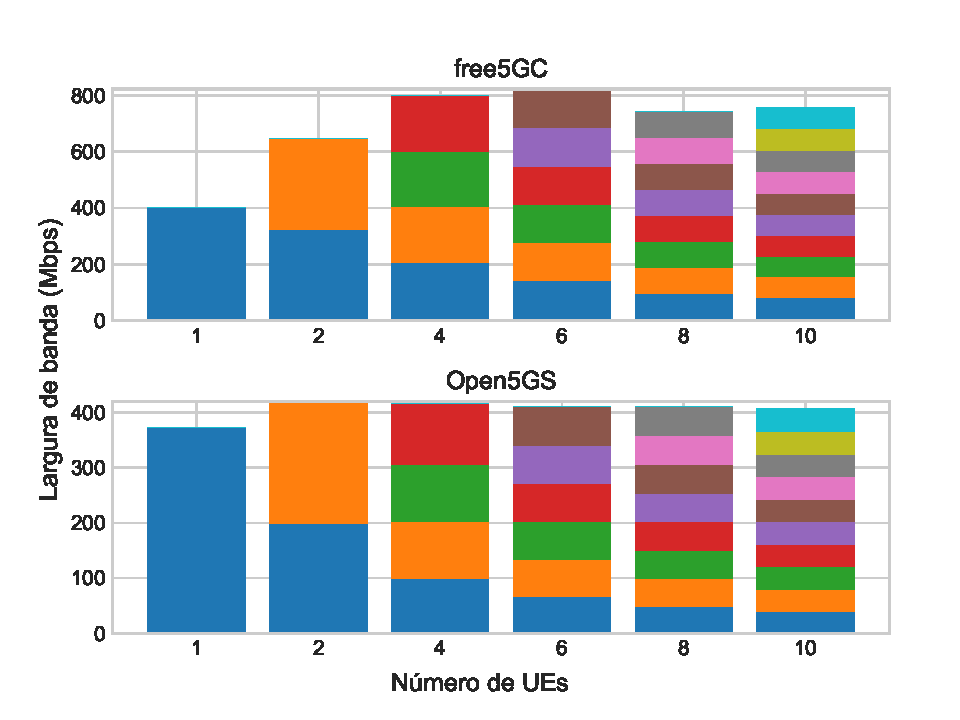
\includegraphics[width=1\textwidth]{TG2/Chapters/DataAnalysis/Figures/EXP2-ALL-6C-8GB.pdf}
    \caption{Valor agregado da largura de banda para cada configuração de quantidade de UEs}
    \label{fig:exp2_all_6-8}
\end{figure}

A Figura \ref{fig:exp2_all_4-4} representa os resultados obtidos para a execução do experimento em uma máquina virtual com 4 núcleos virtuais de processador e 4 GB de memória RAM.
Essa configuração foi utilizada para simular um cenário com recursos limitados.
Neste caso, o desempenho máximo do núcleo \textit{free5GC} ocorre com quatro UEs simultâneos. 
A redução de desempenho para testes com maior quantidade de UEs simultâneos é explicada pela sobrecarga de uso de processador causada pela quantidade de UEs trafegando dados em paralelo.

\begin{figure}[H]
    \centering
    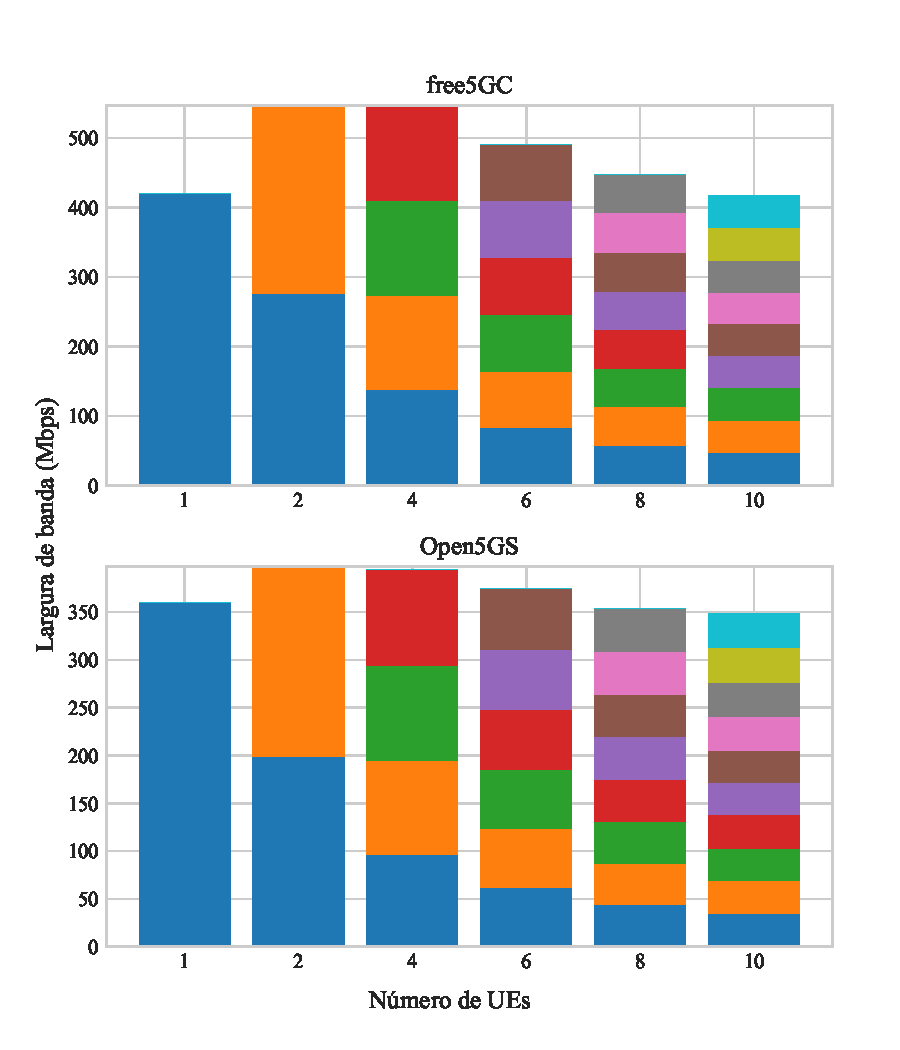
\includegraphics[width=1\textwidth]{TG2/Chapters/DataAnalysis/Figures/EXP2-ALL-4C-4GB.pdf}
    \caption{Valor agregado da largura de banda para cada configuração de quantidade de UEs}
    \label{fig:exp2_all_4-4}
\end{figure}


% \section{Análise e discussão em relação ao consumo de recursos}
% Esta seção apresenta a análise de dados de uso de processador e memória RAM da máquina virtual para a execução dos experimentos.
Os dados para cada contêiner foram agrupados em três conjuntos, para facilitar a visualização dos dados.
O primeiro conjunto representa os dados agregados de todas as instâncias do testador, denominado nos gráficos como Testadores.
O segundo conjunto representa os dados agregados de todas as funções do núcleo em teste, denominado nos gráficos como Núcleo.
O terceiro conjunto representa os dados agregados do restante dos serviços em execução, como os contêineres utilizados para rodar o módulo de coleta de dados do núcleo e o servidor da aplicação \textit{iPerf} utilizada no segundo experimento, denominado nos gráficos como Outros.
Uma análise com maiores detalhes do uso de recursos para cada componente em execução durante o período do experimento é possível ao utilizar a ferramenta para gerar visualizações dos dados coletados disponível através da aplicação \textit{InfluxDB}.
Essa ferramenta faz parte do módulo de coleta de dados do núcleo da rede.

\subsection{Análise e discussão em relação ao consumo de recursos do experimento de registro e estabelecimento de sessão do núcleo 5G}

Para a análise do uso de recursos de processador e memória RAM para a execução do experimento de registro e estabelecimento de sessão do núcleo 5G, foi utilizada uma execução do experimento com intervalo entre conexões de UEs de 500 ms sobre a máquina virtual com 12 núcleos de processador virtuais e 8 GB de memória RAM.
Os resultados agregados podem ser vistos na Figura \ref{fig:exp1_500ms_res}.

\begin{figure}[H]
    \centering
    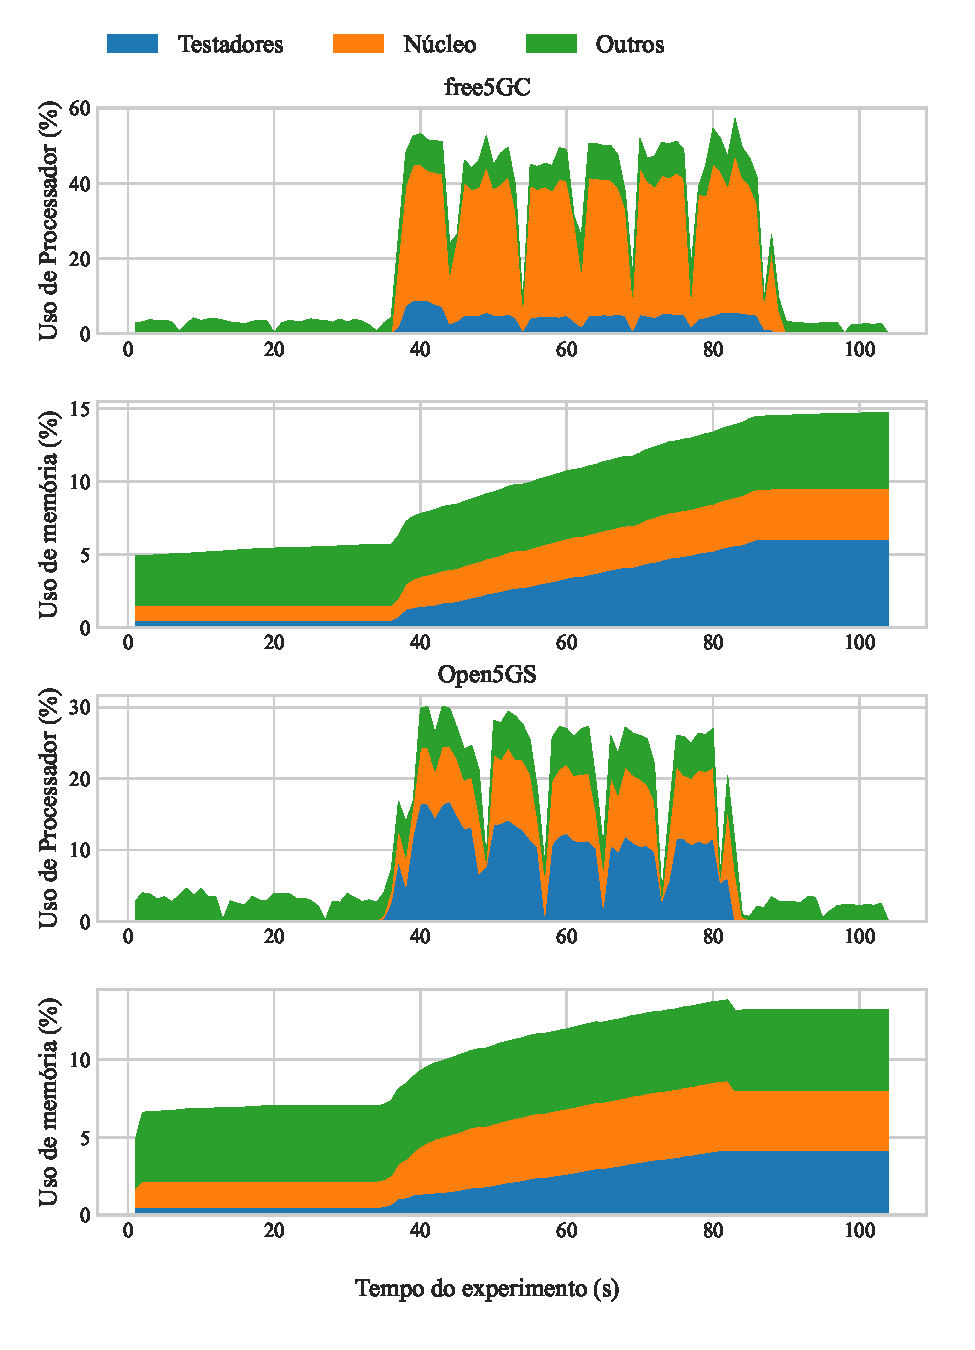
\includegraphics[width=0.95\textwidth]{TG2/Chapters/DataAnalysis/Figures/EXP1-CONN-RES-500ms-12C-8GB.pdf}
    \caption{Uso de processador e memória RAM para a execução com atraso de 500 ms entre conexões}
    \label{fig:exp1_500ms_res}
\end{figure}

Esta figura apresenta o uso de processador e memória RAM de acordo com o tempo de execução do experimento para os núcleos \textit{free5GC} e \textit{Open5GS}.
O eixo X dos gráficos representam o tempo em segundos referente à coleta de dados total do experimento, considerando o tempo para a inicialização, execução e encerramento do experimento.
O eixo Y representa a porcentagem do uso para cada tipo de recurso analisado.
As áreas azuis, laranjas e verdes dos gráficos representam a porcentagem de uso agregado de recursos para a execução dos testadores, núcleos 5G e os demais componentes, respectivamente.

Ao observar o uso de recursos somente durante o período da execução do experimento, a média de uso de processador para o núcleo \textit{free5GC} foi de 31,33\% e para o núcleo \textit{Open5GS} foi de 7,26\%.
Em relação ao uso de memória RAM, o pico de uso de memória para o núcleo \textit{free5GC} foi de 3.45\%, representando o uso de 282,6 MB de memória RAM.
Quanto ao núcleo \textit{Open5GS}, o pico de uso de memória RAM foi de 4,47\%, representando o uso de 366,2 MB de memória RAM.
Os resultados descritos acima demonstram que o núcleo de rede 5G \textit{Open5GS} apresentou uma performance 4.3x superior em relação ao uso de processador em comparação com o núcleo \textit{free5GC}.
Entretanto, em relação ao uso de memória RAM, o núcleo \textit{free5GC} apresentou uma performance 1.29x superior ao núcleo \textit{Open5GS}.


\subsection{Análise e discussão em relação ao consumo de recursos do experimento de desempenho do plano de dados}

Para realizar a análise do uso de recursos durante a execução do experimento para a avaliação do desempenho do plano de dados, foi escolhida as métricas de uso de recursos do processador e memória RAM.
Essa análise complementa a explicação do experimento demonstrada na Seção \ref{sec:results-dataplane-analysis}.
Os experimentos foram conduzidos em quatro configurações diferentes.
Entretanto, a análise do consumo de recursos foi focada em apenas duas configurações, com a maior e com a menor quantidade de recursos.
Ao observar os resultados do plano de dados para a execução do experimento de desempenho do plano de dados na máquina virtual com 12 núcleos virtuais e 8 GB de memória RAM, percebe-se que o desempenho máximo para o plano de dados do núcleo \textit{free5GC} com essa configuração de máquina virtual não foi atingido.
Esse resultado pode ser visto nos gráficos da Figura \ref{fig:exp2_10gnb_12c}.


\begin{figure}[H]
    \centering
    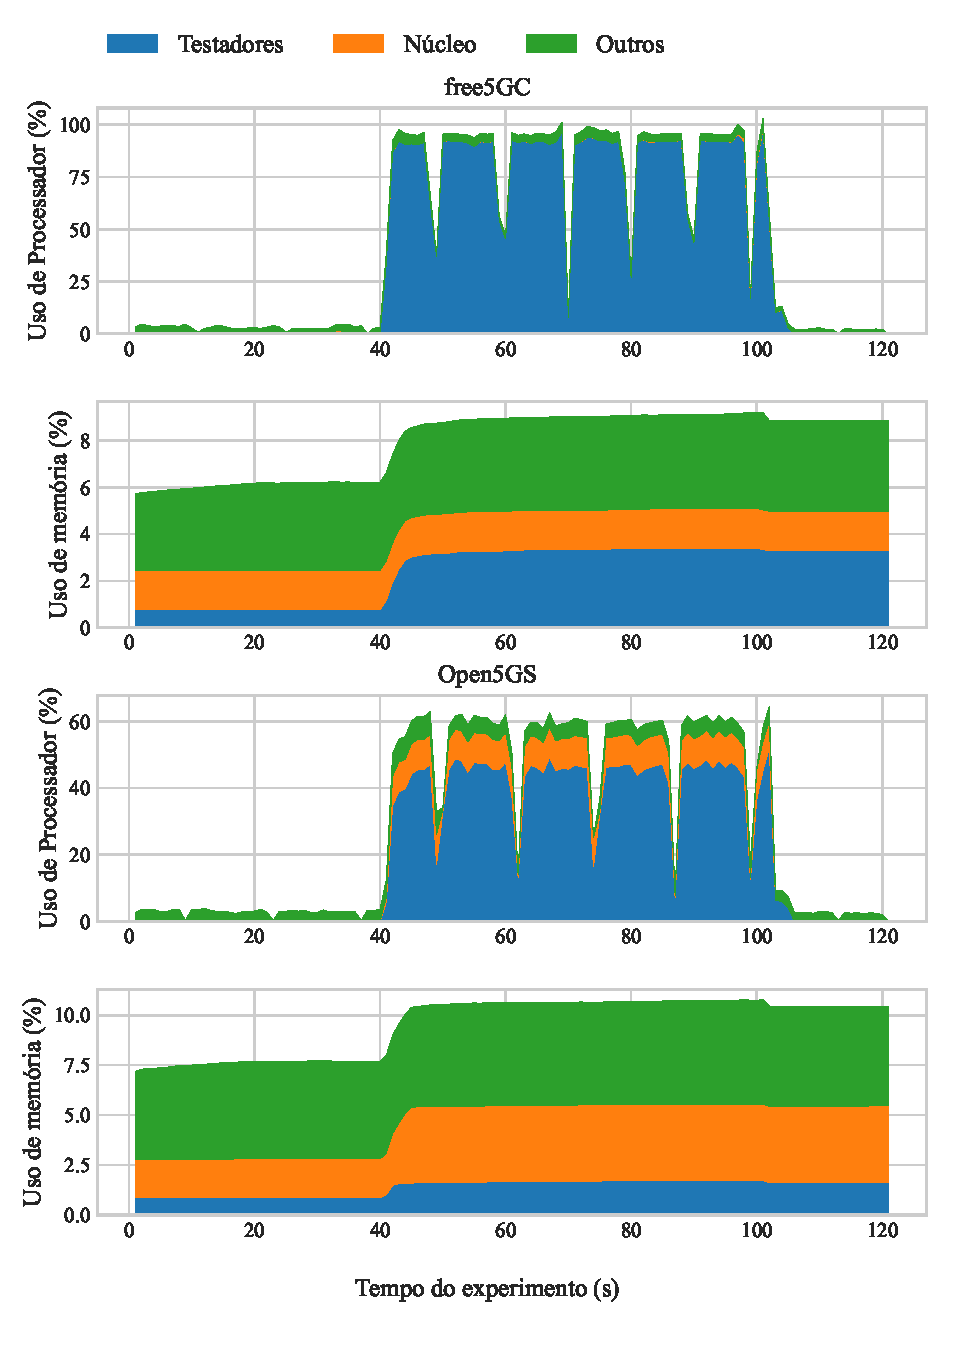
\includegraphics[width=0.95\textwidth]{TG2/Chapters/DataAnalysis/Figures/EXP2-IPERF-RES-10gNB-12C-8GB.pdf}
    \caption{Uso de processador e memória RAM para o experimento de desempenho de plano de dados com 10 UEs conectados}
    \label{fig:exp2_10gnb_12c}
\end{figure}

É possível observar que o uso médio de processador durante a execução desse experimento foi de 95,57\% para o núcleo \textit{free5GC}, com poucos picos de uso atingindo os 100\%.
Do total de uso de processador, 91,87\% do uso é representado pelos testadores e UEs realizando os testes.
O uso de processador médio do núcleo \textit{free5GC} durante a execução do experimento foi de 0,03\%.
Isso demonstra que o núcleo de rede 5G utiliza poucos recursos de processador para realizar o gerenciamento do plano de dados dos UEs conectados.

Em relação ao núcleo \textit{Open5GS}, que não é otimizado para o gerenciamento do plano de dados de múltiplos UEs em paralelo, o uso de processador médio total durante a execução do experimento foi de 59,59\%.
O total de uso de processador durante a execução de experimento é dividida principalmente entre as instâncias do testador e o núcleo da rede 5G, com o testador representando 45,95\% do uso do processador e o núcleo representando 8,96\%.
A redução de uso de processador pelas instâncias do testador e UEs em relação ao experimento executado com o núcleo \textit{free5GC} é explicada pela baixa largura de banda disponível pelo \textit{Open5GS}.

Uma possível explicação desses resultados é que o núcleo \textit{free5GC} provavelmente utiliza paralelização para gerenciar o processamento do plano de dados dos UEs.
Isso provavelmente justificaria a facilidade em escalar a quantidade de UEs conectados reduzindo sutilmente o desempenho individual dos UEs.
Por outro lado, o núcleo \textit{Open5GS} não apresenta o mesmo comportamento.
De acordo com os resultados, o núcleo utilizou 8,96\% do total de processamento disponível na máquina virtual.
Isso é equivalente a um pouco mais que a capacidade de um núcleo do processador disponível.
Possivelmente, este núcleo não está otimizado para paralelizar o processamento do plano de dados quando múltiplos UEs estão conectados.
Isso explicaria o baixo desempenho observado nos resultados do núcleo \textit{Open5GS}.

Ao observar o uso de recursos de processador para a máquina virtual com 4 núcleos virtuais de processador e 4 GB de memória RAM, é possível explicar a queda de desempenho para o plano de dados do núcleo \textit{free5GC} após os testes com mais de 4 UEs simultâneos.
A Figura \ref{fig:exp2_4gnb_4c} representa os gráficos de uso de processador e memória RAM para uma execução do experimento de desempenho do plano de dados 

\begin{figure}[H]
    \centering
    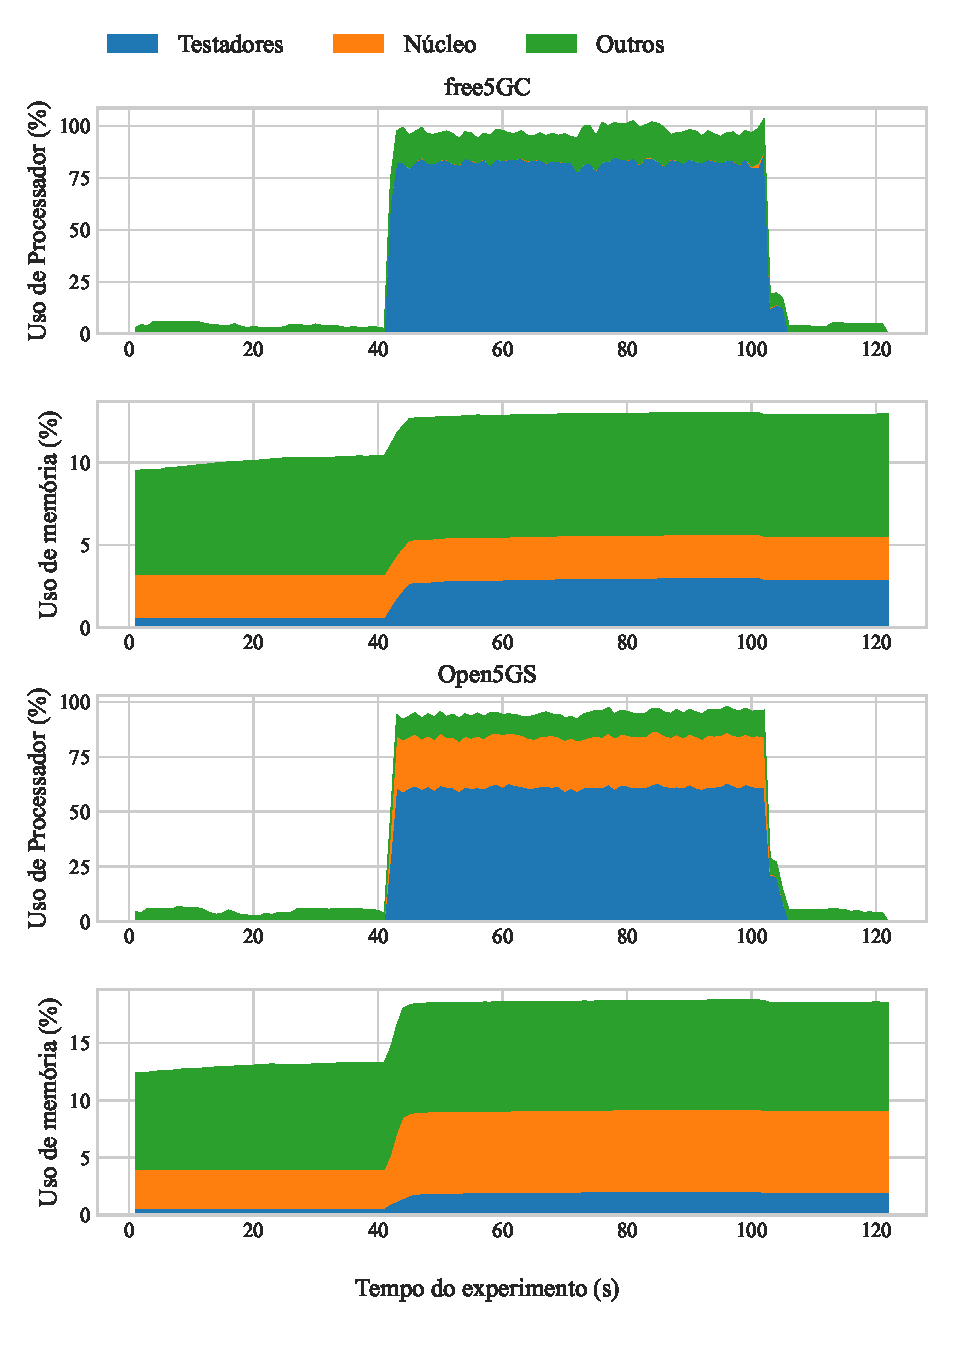
\includegraphics[width=0.95\textwidth]{TG2/Chapters/DataAnalysis/Figures/EXP2-IPERF-RES-4gNB-4C-4GB.pdf}
    \caption{Uso de processador e memória RAM para o experimento de desempenho de plano de dados com 4 UEs conectados}
    \label{fig:exp2_4gnb_4c}
\end{figure}

É possível observar que o uso do processador para a execução de quatro UEs conectados e utilizando o plano de dados do núcleo de rede 5G \textit{free5GC} está muito próximo de 100\%, atingindo o uso máximo do processador em diversos momentos.
Dessa forma, é possível perceber que o máximo de UEs simultâneos que essa configuração de máquina virtual suporta são quatro.
Para quantidades superiores a quatro UEs simultâneos, a redução de desempenho do plano de dados é explicada devido ao chaveamento necessário realizado pelo sistema operacional para gerenciar os diversos processos executando em paralelo.




% Livro sobre análise de dados:
% https://app.minhabiblioteca.com.br/reader/books/9788584291434/pageid/28
